\chapter{Badane algorytmy}

\section{Wprowadzenie}
Niniejszy rozdział opisuje algorytmy dla funkcji dominowania rzymskiego słabo spójnego. Analizowane one będą pod kątem złożoności, wydajności, poprawności oraz potencjalnego zastosowania. Wszystkie algorytmy wyznaczają dodatkowo zbiór dominowania rzymskiego słabo spójnego. Lista analizowanych algorytmów jest następująca:

\begin{itemize}
    \item algorytm brute force
    \item algorytm liniowy dla drzew
    \item algorytm programowania liniowego I
    \item algorytm programowania liniowego II
    \item algorytm mrówkowy
    \item algorytm aproksymacyjny
    \item algorytm zachłanny
\end{itemize}

\section{Algorytm Brute Force}

\subsection{Działanie}
Jest to w zasadzie trywialna implementacja dokładnego algorytmu wyznaczającego funkcję oraz zbiór dominujący rzymski słabo spójny poprzez sprawdzenie każdej kombinacji wartości \{0, 1, 2\} na wierzchołkach grafu wejściowego. Każda kombinacja sprawdzana jest pod względem poprawności według definicji słabo spójności w następujący sposób:
\begin{itemize}
    \item wyznaczamy zbiór indukowany, który składa się ze zbioru dominującego (wierzchołki z wartościami \{1, 2\}) oraz sąsiadów wierzchołków zbioru dominującego,
    \item sprawdzamy czy wszystkie wierzchołki z wartością 0 mają sąsiada z wartością 2,
    \item dla każdego wierzchołka ze zbioru indukowanego dodajemy krawędzie, ale tylko te wychodzące z wierzchołków zbioru dominującego
    \item następnie sprawdzamy, czy powstały graf jest spójny. Jeśli jest, to zbiór spełnia założenia definicji.
\end{itemize}

\subsection{Złożoność i wydajność}

Algorytm ma złożoność wykładniczą, zatem nie będzie wykonywalny w rozsądnym czasie dla większych grafów.
\begin{itemize}
    \item generowanie wszystkich kombinacji możliwych przypisań: $3^n$, gdzie $n$ to liczba wierzchołków grafu,
    \item sprawdzanie własności zbioru słabo spójnego dla każdego przypisania: $n^2$
\end{itemize}

Zatem złożoność czasowa algorytmu wynosi $O(3^n \cdot n^2)$\\
Złożoność pamięciowa ogranicza się do przechowywania grafu w pamięci i wynosi $O(n + m)$

\subsection{Pseudokod}

\begin{algorithm}
    \caption*{Algorytm Brute Force}
    \begin{algorithmic}[1]
        \Function{FindRomanDominatingSet}{graph}
            \State Initialize $min\_roman\_number \gets \infty$
            \State Initialize $best\_node\_values \gets None$
            \State $nodes \gets$ list of nodes in $graph$
    
            \For{each assignment of values $(0,1,2)$ to all nodes}
                \State $node\_values \gets$ mapping of nodes to values
                
                \For{each node in graph} \Comment{Sprawdzanie warunku dominacji}
                    \If{$node\_values[node] = 0$}
                        \If{\textbf{not} any neighbor of $node$ has value $2$}
                            \State \textbf{Continue} to next assignment
                        \EndIf
                    \EndIf
                \EndFor
                
                \State $induced\_set \gets$ nodes with values $\{1,2\}$
    
                \For{each node in $induced\_set$}
                    \State Add all its neighbors to $induced\_set$
                \EndFor
    
                \State Create empty $induced\_graph$
                \For{each node in $induced\_set$}
                    \If{$node\_values[node]$ is $1$ or $2$}
                        \For{each neighbor in $graph$}
                            \If{neighbor in $induced\_set$}
                                \State Add edge to $induced\_graph$
                            \EndIf
                        \EndFor
                    \EndIf
                \EndFor
    
                \If{$induced\_graph$ is connected}
                    \State Compute $roman\_number \gets$ sum of $node\_values$
                    \If{$roman\_number < min\_roman\_number$}
                        \State Update $min\_roman\_number$ and $best\_node\_values$
                    \EndIf
                \EndIf
            \EndFor
    
            \State \Return $(min\_roman\_number, best\_node\_values)$
        \EndFunction
    \end{algorithmic}
\end{algorithm}

\section{Algorytm liniowy dla drzew}

\subsection{Działanie}

Dla każdego wierzchołka definiujemy następujące parametry:
\begin{itemize}
    \item $v['R']$ - wartość funkcji dominowania rzymskiego słabo spójnego w wierzchołku $v$, z założeniem, że $v['R']\in\{0,1,2\}$
    \item $v['n00']$ - oznacza liczbę dzieci z $R=0$ oraz bez sąsiada z $R=2$ (dziecko niezdominowane)
    \item $v['n01']$ - oznacza liczbę dzieci z $R=0$ i z sąsiadem z $R=2$ (dziecko zdominowane)
    \item $v['n1']$ - oznacza liczbę dzieci wierzchołka $v$ z $R = 1$
    \item $v['n2']$ - oznacza liczbę dzieci wierzchołka $v$ z $R = 2$
    \item $v['sw']$ - oznacza liczbę dzieci wierzchołka $v$ z $n00=1$ i $n01=0$. (wierzchołek wspierający)
    \item $v['ch'] =1$ jeśli $v['sw']>1$ lub jeśli $v['sw']=1$ i mający przynajmniej jedno dziecko z $R=0$; w przeciwnym razie $v['ch'] =0$. Jeśli $v['ch'] =1$, wtedy $v['R']=2$ i w Fazie~2 każde dziecko $v$ z $n00=1$ i z $n01=0$ dostaje $R=0$ i jego jedyne dziecko z $R=0$ zmienia wartość na $R=1$.
    \item $v['child']$ - jeśli $v$ jest wierzchołkiem wspierającym, wtedy wartość ta jest numerem liścia sąsiadującego z $v$.
\end{itemize}

Algorytm ma 2 fazy. W obu fazach rozpatrujemy wszystkie wierzchołki drzewa według odwrotnego porządku drzewa, czyli od ostatniego wierzchołka do korzenia (reverse tree-order). Wszystkie poczatkowo zdefiniowane wartości mają wartości 0. W bardzo ogólnym rozumieniu, rozpatrujemy każdy wierzchołek na podstawie sąsiedztwa, relacji ojciec-dziecko oraz wartości zdefiniowanych parametrów i aktualizację ich w obu fazach. Wartości $R$ przy każdym wierzchołku, to wartości dominowania rzymskiego słabo spójnego, a suma tych wartości to funkcja dominowania rzymskiego słabo spójnego.
\\
Z racji sporego stopnia skomplikowania algorytmu, jego działanie zostanie przedstawione na przykładzie.
Dany jest graf $G$ będący drzewem ukorzenionym o 10 wierzchołkach, ponumerowanych wartościami od 0 do 9. Zakładamy, że wyznaczenie ojca każdego z wierzchołków jest trywialne i niezłożone czasowo, dlatego podczas rozważań wyznaczanie ojca wierzchołka będzie pomijane.

\begin{figure}[H]
    \centering
    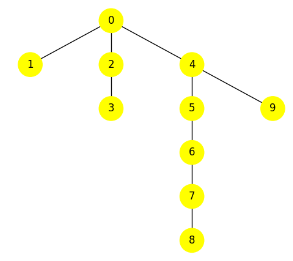
\includegraphics[width=0.5\textwidth]{assets/image.png}
    \caption{Graf $G$ - przykładowe drzewo}
    \label{fig:drzewo}
\end{figure}

\begin{enumerate}
    \item Jeśli wierzchołek jest liściem i nie jest korzeniem to zwiększamy wartość 'n00' ojca o 1.\\
    Zatem dla liści 1,3,8,9, wartości ich ojców wyglądają następująco:\\
        T[7]['n00'] = 1  \\
        T[7]['child'] = 8  (od wierzchołka 8)\\
        T[4]['n00'] = 1 \\
        T[4]['child'] = 9  (od wierzchołka 9)\\
        T[2]['n00'] = 1  \\
        T[2]['child'] = 3  (od wierzchołka 3)\\
        T[0]['n00'] = 1 \\
        T[0]['child'] = 1  (od wierzchołka 1)
    \item Jeśli wierzchołek nie jest liściem:
    \begin{enumerate}
        \item Sprawdzamy czy wierzchołek posiada tylko jedno niezdominowane dziecko i posiada ojca. W tym przypadku ojciec będzie wierzchołkiem wspierającym. \\
        T[6]['sw'] = 1 (od wierzchołka 7)\\
        T[0]['sw'] = 2 (od wierzchołka 4 i 2)
        \item Sprawdzamy sumę wartości dzieci zdominowanych, niezdominowanych oraz liczbę dzieci dla których wierzchołek jest wspierający. Jeśli ta suma jest większa od 1, to wartość tego wierzchołka ustawiamy na 2, a parametr 'ch' na 1.\\
        T[0]['R'] = 2  (od wierzchołka 0)\\
        T[0]['ch'] = 1  (od wierzchołka 0)
        \begin{enumerate}
            \item Jeśli wierzchołek ma ojca to parametr 'n2' ojca zwiększamy o 1, a jeśli wierzchołek posiada tylko jedno niezdominowane dziecko zmniejszamy parametr wspierający u ojca.
        \end{enumerate}
        \item Jeśli wierzchołek nie jest wspierający:
            \begin{enumerate}
                \item Jeśli wierzchołek posiada niezdominowane dzieci lub jedno dziecko i żadnych dzieci z wartością 2 lub dzieci zdominowane, to wtedy wierzchołek będzie miał wartość 2. Dla istniejącego ojca wierzchołka zwiększamy 'n2'.\\
                T[7]['R'] = 2  (od wierzchołka 7)\\
                T[6]['n2'] = 1  (od wierzchołka 7)\\
                T[4]['R'] = 2  (od wierzchołka 4)\\
                T[0]['n2'] = 2  (od wierzchołka 4 i 2)\\
                T[2]['R'] = 2  (od wierzchołka 2)\
                \item Jeśli wierzchołek posiada niezdominowane dziecko, to danemu wierzchołkowi przypisujemy wartość 0, a temu dziecku wartość 1, a dla ojca zmniejszamy wartość wspierania.
                \item Jeśli wierzchołek posiada tylko dzieci zdominowane, to danemu wierzchołkowi przypisujemy wartość 1, a ojcu zwiększamy wartość 'n1'.\\
                T[5]['R'] = 1  (od wierzchołka 5)\\
                T[4]['n1'] = 1  (od wierzchołka 5)
            \end{enumerate}
        \item Jeśli wartość wierzchołka wynosi 0, posiada on dzieci z wartością 2 oraz ojca, to zwiększamy wartość ojca 'n01' o 1,\\
        T[5]['n01'] = 1  (od wierzchołka 6)
        \item Jeśli wartość wierzchołka wynosi 0, nie posiada on dzieci z wartością 2 oraz ojca, to zwiększamy wartość ojca 'n00' o 1,\\
    \end{enumerate}
    \item Korzeń należy rozpatrzeć dodatkowo. Jeśli nie posiada on dzieci z wartościami 2 i sam ma wartość 0, to przypisujemy mu $R=2$,
    \item Jeśli liczba dzieci korzenia z $R=1$ jest równa liczbie dzieci pomniejszonej o 1, to korzeń również ma wartość 1.
\end{enumerate}

Zdjęcie przedstawia zachowanie algorytmu po fazie 1. Czerwone wierzchołki to wartość $R=2$, niebieskie to $R=1$, a żółte to $R=0$. Widać, że przypisanie nie jest jeszcze optymalne.

\begin{figure}[H]
    \centering
    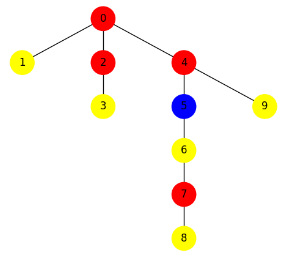
\includegraphics[width=0.5\textwidth]{assets/phase1.png}
    \caption{Graf $G$ - po fazie 1}
    \label{fig:drzewoFaza1}
\end{figure}

W fazie 2, dla każdego wierzchołka posiadającego ojca, tylko jedno dziecko niezdominowane i parametr ojca 'ch' wynoszący 1, wtedy musimy ,zmienić' układ, poprzez ustawienie 0 na obecnym wierzchołku, ustawienie dziecka na 1 oraz zwiększenie liczby dzieci niedominowanych ojca wierzchołka. 
Ten warunek spełniony jest dla wierzchołków 4 i 2. Zatem:\\
T[4]['R'] = 0  (od wierzchołka 4)\\
T[9]['R'] = 1  (dziecko wierzchołka 4)\\
T[2]['R'] = 0  (od wierzchołka 2)\\
T[3]['R'] = 1  (dziecko wierzchołka 2)\\
T[0]['n00'] = 3  (ojciec wierzchołków 4 i 2)

Poniższy rysunek przedstawia prawidłowe przypisanie wartości $R$ po fazie 2.\\

\begin{figure}[H]
    \centering
    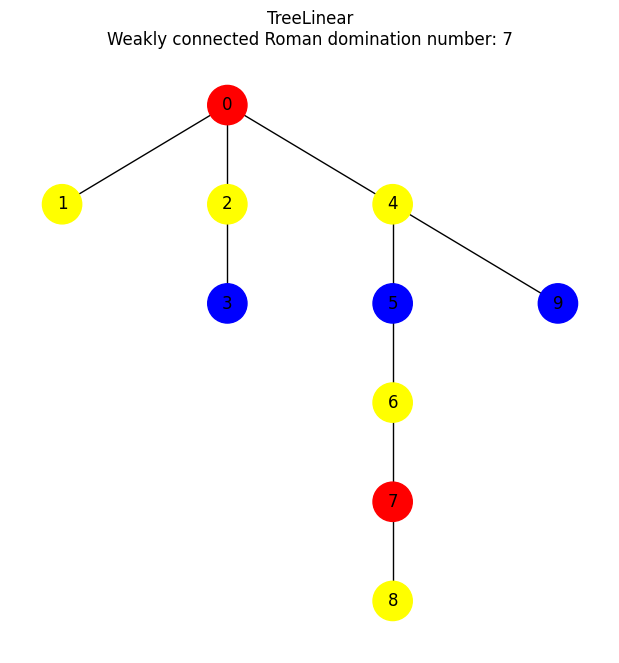
\includegraphics[width=0.5\textwidth]{assets/phase2.png}
    \caption{Graf $G$ - po fazie 2 - finalna wersja}
    \label{fig:drzewoFaza2}
\end{figure}

\subsection{Złożoność i wydajność}
Algorytm ma złożoność liniową $O(n)$, gdzie n to liczba wierzchołków drzewa. Algorytm zatem jest skalowalny i szybki dla większych grafów, natomiast ograniczony do jednej ich klasy - drzew.

\subsection{Pseudokod}
\begin{algorithm}
    \caption*{Algorytm liniowy dla drzew - Faza 1}
    \begin{algorithmic}[1]
        \Function{Phase1}{T, root}
            \State $father\_map \gets$ Compute parent-child relationships using BFS
            \State $nodes\_ids \gets$ List of all nodes in $T$
    
            \For{each node $v$ in reversed($nodes\_ids$)}
                \State $father \gets father\_map[v]$
    
                \If{$v$ is a leaf and $v \neq root$}
                    \State Increase $T[father]['n00']$
                    \State Set $T[father]['child'] \gets v$
                \Else
                    \If{$T[v]['n00'] == 1$ and $T[v]['n01'] == 0$ and $father$ exists}
                        \State Increase $T[father]['sw']$
                    \EndIf
    
                    \If{$T[v]['sw'] + T[v]['n00'] + T[v]['n01'] > 1$}
                        \State Set $T[v]['R'] = 2$
                        \If{$father$ exists}
                            \State Increase $T[father]['n2']$
                            \If{$T[v]['n00'] == 1$ and $T[v]['n01'] == 0$}
                                \State Decrease $T[father]['sw']$
                            \EndIf
                        \EndIf
                        \State $T[v]['ch'] = 1$
                    \EndIf
    
                    \If{$T[v]['sw'] == 0$}
                        \If{$T[v]['n00'] > 1$ or ($T[v]['n00'] == 1$ and ($T[v]['n2'] == 0$ or $T[v]['n01'] > 0$))}
                            \State Set $T[v]['R'] = 2$
                            \If{$father$ exists}
                                \State Increase $T[father]['n2']$
                            \EndIf
                        \ElsIf{$T[v]['n00'] == 1$}
                            \State Set $T[v]['R'] = 0$
                            \State Set $T[T[v]['child']]['R'] = 1$
                            \If{$father$ exists}
                                \State Decrease $T[father]['sw']$
                            \EndIf
                        \EndIf
                        \If{$T[v]['n00'] == 0$ and $T[v]['n01'] > 0$}
                        \State Set $T[v]['R'] = 1$
                        \If{$father$ exists}
                            \State Increase $T[father]['n1']$
                        \EndIf
                    \EndIf
                    \EndIf
                    \If{$T[v]['R'] = 0$ \textbf{and} $T[v]['n2'] > 0$ \textbf{and} $father$ exists}
                        \State $T[father]['n01'] \gets T[father]['n01] + 1$
                    \EndIf

                    \If{$T[v]['R'] = 0$ \textbf{and} $T[v]['n2'] = 0$ \textbf{and} $father$ exists}
                        \State $T[father]['n00'] \gets T[father]['n00] + 1$
                    \EndIf

                \EndIf
            \EndFor
    
            \If{$T[root]['n2'] == 0$ and $T[root]['R'] == 0$}
                \State Set $T[root]['R'] = 2$
            \EndIf
            \If{$T[root]['n1'] ==$ (number of root's neighbors - 1)}
                \State Set $T[root]['R'] = 1$
            \EndIf
    
            \State \Return $T$
        \EndFunction
    \end{algorithmic}
    \end{algorithm}
    
    \begin{algorithm}
    \caption*{Algorytm liniowy dla drzew - Faza 2}
    \begin{algorithmic}[1]
        \Function{Phase2}{T, root}
            \For{each node $v$ in reversed($nodes\_ids$)}
                \State $father \gets father\_map[v]$
                \If{$father$ exists}
                    \If{$T[v]['n00'] == 1$ and $T[father]['ch'] == 1$ and $T[v]['n01'] == 0$}
                        \State Set $T[v]['R'] = 0$
                        \State Set $T[T[v]['child']]['R'] = 1$
                        \State Increase $T[father]['n00']$
                    \EndIf
                \EndIf
            \EndFor
    
            \State \Return $T$
        \EndFunction
    \end{algorithmic}
\end{algorithm}

\FloatBarrier
\section{Algorytm programowania liniowego I}
Jest to algorytm programowania liniowego zaimplementowany na podstawie artykułu ,,Algorithmic complexity of weakly connected Roman domination in graphs" \cite{ILP}.

\subsection{Działanie}

Ten model programowania liniowego wymagania zdefiniowania następujących zmiennych:

\[
x_e =
\begin{cases}
1, & e \in E' \\
0, & e \notin E'
\end{cases}
\quad
y_e =
\begin{cases}
1, & e \in T' \\
0, & e \notin T'
\end{cases}
\]

\[
a_v =
\begin{cases}
1, & v \in V_1 \cup V_2 \\
0, & v \in V_0
\end{cases}
\quad
b_v =
\begin{cases}
1, & v \in V_2 \\
0, & v \in V_0 \cup V_1
\end{cases}
\]

gdzie \( v \in V \), \( e \in E \) i \( T' \) to drzewo rozpinające podgrafu \( G' \).

Definiujemy funkcję celu, czyli minimalizację wagi zbioru dominującego rzymskiego słabo spójnego:

\[
\text{Z: } \min \left( \sum_{v \in V} a_v + \sum_{v \in V} b_v \right)
\]

oraz ograniczenia:\\
Wierzchołek o wartości 0, bedzie miał przynajmniej jednego sasiada z wartością 2:
\[
    a_v + \sum_{k \in N_G(v)} b_k \geq 1, \quad v \in V, \tag{1}
\]
Krawędź istnieje w drzewie rozpinającym \( T' \), jesli ta krawędź należy do \( G' \). Ograniczenie to zapewnia spójność w \( G' \):
\[
    y_e \leq x_e, \quad e \in E, \tag{2}
\]
Wybór krawędzi, które mają  wartość należącą do zbioru dominującego na przynajmniej jednym swoim końcu:
\[
    x_e \leq a_{i_e} + a_{j_e}, \quad e \in E_{G'}, \tag{3}
\]
Drzewo rozpinające \( T' \) ma liczbę krawędzi równą liczbie wierzchołków grafu pomniejszoną o 1:
\[
    \sum_{e \in E} y_e = n - 1, \tag{4}
\]
Drzewo rozpinające \( T' \) nie posiada cykli:
\[
    \sum_{i_e, j_e \in S} y_e \leq |S| - 1, \quad S \subseteq V, \quad |S| \geq 3, \tag{5}
\]
Podzbior wierzchołków z $b_v = 1$, czyli $(V_2)$, jest podzbiorem wierzchołków z $a_v = 1$, czyli $(V_1 \cup V_2)$
\[
    b_v \leq a_v, \quad v \in V. \tag{6}
\]

Warunki 1, 2, 5 gwarantują, że \( T' \) jest drzewem rozpinającym grafu \( G' \).

\subsection{Złożoność i wydajność}

Liczba zmiennych dla grafu o $n$ wierzchołkach i $m$ krawędziach wynosi $O(n+m)$.
Z powodu wykładniczej natury nierówności liczba ograniczeń wynosi $O(2^n)$.

\subsection{Pseudokod}

\begin{algorithm}
    \caption*{Algorytm programowania liniowego I}
    \begin{algorithmic}[1]
        \Function{ILP\_I}{graph}
            \State $V \gets$ list of nodes in $graph$
            \State $E \gets$ list of edges in $graph$
    
            \State Initialize ILP model $model$
            \State Set objective: Minimize $\sum (a[i] + b[i])$ for all nodes $i \in V$
    
            \State Define binary variables:

            \State $x[i, j]$ for $(i, j) \in E$ \Comment{1 jeśli krawędź jest w $G'$}
            \State $y[i, j]$ for $(i, j) \in E$ \Comment{1 jeśli krawędź jest w drzewie rozpinającym $T'$}
            \State $a[i]$ for $i \in V$ \Comment{1 jeśli wierzchołek należy do $V1 \cup V2$}
            \State $b[i]$ for $i \in V$ \Comment{1 jeśli wierzchołek należy do $V2$}
    
            \State \textbf{Constraints:}
    
            \For{each node $i$ in $V$} \Comment{Każdy wierzchołek musi być broniony}
                \State Add constraint: $a[i] + \sum b[k] \geq 1$, where $k$ are neighbors of $i$
            \EndFor
    
            \For{each edge $(i, j)$ in $E$}
                \State Add constraint: $y[i, j] \leq x[i, j]$ \Comment{Krawędź drzewa musi istnieć w $G'$}
                \State Add constraint: $x[i, j] \leq a[i] + a[j]$ \Comment{Krawędzie drzewa muszą łączyć bronione wierzchołki}
            \EndFor
    
            \State Add constraint: $\sum y[i, j] = |V| - 1$ \Comment{Drzewo musi mieć $|V| - 1$ krawędzi}
    
            \State Find cliques of size $\geq 3$ in $graph$ and store as $subsets$
            \For{each subset $S$ in $subsets$} \Comment{Eliminacja cykli}
                \State Add constraint: $\sum y[i, j] \leq |S| - 1$ for edges $(i, j) \in S$
            \EndFor
    
            \For{each node $i$ in $V$} \Comment{Wierzchołki z $V2$ muszą należeć do $V1 \cup V2$}
                \State Add constraint: $b[i] \leq a[i]$
            \EndFor
    
            \State Solve ILP model
    
            \State Extract solution:
            \For{each node $i$ in $V$}
                \State $solution[i] \gets round(a[i].X) + 2 * round(b[i].X)$
            \EndFor
    
            \State \Return $(model.objVal, solution)$
        \EndFunction
    \end{algorithmic}
\end{algorithm}

\FloatBarrier
\section{Algorytm programowania liniowego II}
Jest to algorytm programowania liniowego zaimplementowany na podstawie artykułu ,,Algorithmic complexity of weakly connected Roman domination in graphs" \cite{ILP}, podobnie jak poprzedni.
\subsection{Działanie}
Model ten opiera się na przepływach. W tym modelu rozpatrujemy graf jako wierzchołek który zużywa jednostkę przepływu, przepływając przez krawędzie grafu. Na wejściu definiujemy zewnętrzny przepływ, którego liczba jednostek jest równa liczbie wierzchołków grafu. Zachowujemy zasadę przepływu sieci, dlatego próbujemy wprowadzić przepływ zewnętrzny w jak najwiekszej ilości przez pojedynczy wierzchołek.\\
Definiujemy następujące zmienne:
\[
x_i =
\begin{cases}
1, & i \in V_1 \cup V_2 \\
0, & i \in V_0
\end{cases}
\quad
y_i =
\begin{cases}
1, & i \in V_2 \\
0, & i \in V_0 \cup V_1
\end{cases}
\]

\[
a_e =
\begin{cases}
1, & e \in E' \\
0, & e \notin E'
\end{cases}
\quad
t_i =
\begin{cases}
1, & \text{wierzchołek korzenia} = i \\
0, & \text{pozostałe wierzchołki}
\end{cases}
\]

\[
u_i \in N \cup \{0\}, \quad v_e \in [-n, n].
\]
gdzie:\\
$t_i$ zdefiniowany dla każdego wierzchołka grafu. Identyfikuje, gdzie zewnetrzny wierzchołek jest traktowany jako wejście. \\
$u_i$ reprezentuje liczbę jednostek przepływu zewnętrznego dla danego wierzchołka grafu.\\
$v_e$ oznacza jednostki przepływające przez dane krawędzie.\\
$x_i, y_i$ oznaczają przynależność do zbioru dominującego rzymskiego słabo spójnego.

Minimalizującą liczbę dominowania rzymskiego słabo spójnego jako funkcję celu definiujemy następująco:

\[
\text{Z: } \min \left( \sum_{i \in V} x_i + \sum_{i \in V} y_i \right),
\]

mając dane ograniczenia:\\
Wierzchołek z wartością 0 sąsiaduje z przynajmniej jednym wierzchołkiem z wartością 2:
\[
x_i + \sum_{j \in N_G(i)} y_j \geq 1, \quad i \in V, \tag{1}
\]
Prawidłowe zdefiniowanie zmiennych $x$ i $y$:
\[
y_i \leq x_i, \quad i \in V, \tag{2}
\]
Krawędź $e \in E'$ ma przynajmniej jeden koniec z wierzchołkiem o wartości przynajmniej 1:
\[
a_e \leq x_{i_e} + x_{j_e}, \quad e \in E, \tag{3}
\]
Jest tylko jeden wierzchołek w grafie $G'$ gdzie jest dostarczony przepływ zewnętrzny:
\[
\sum_{i \in V} t_i = 1, \tag{4}
\]
Wielkość przepływu wielkości co najwyżej $n$:
\[
u_i \leq n \cdot t_i, \quad i \in V, \tag{5}
\]
Przepływ ma miejsce tylko w krawędziach należących do $E'$:
\[
v_e \leq n \cdot a_e, \quad e \in E, \tag{6}
\]

\[
v_e \geq -n \cdot a_e, \quad e \in E, \tag{7}
\]
Reprezentacja zasady zachowania sieci:
\[
u_i + \sum_{e: j_e = i} v_e - \sum_{e: i_e = i} v_e = 1, \quad i \in V, \tag{8}
\]
Każdy wierzchołek $v \in V$ musi mieć przynajmniej jeden ustalony wierzchołek w $E'$
\[
a_e \geq 1, \quad e \in E, \tag{9}
\]

\subsection{Złożoność i wydajność}

Suma zmiennych w sformułowanym modelu wynosi $3n + m$, będących wartościami logicznymi, $n$ integralnych i $m$ ciągłych.\\
Liczba ograniczeń wynosi $7n+3m+2$. Wynika to z tego, że nie wszystkie ograniczenia to są nierówności.

\subsection{Pseudokod}
\begin{algorithm}
    \caption*{Algorytm programowania liniowego II}
    \begin{algorithmic}[1]
        \Function{ILP\_II}{graph}
            \State Initialize ILP model $model$ with minimization objective
    
            \State $V \gets$ list of nodes in $graph$
            \State $E \gets$ list of edges in $graph$
            \State $n \gets |V|$ \Comment{Liczba wierzchołków}
    
            \State Define binary variables:

            \State $x[i]$ for $i \in V$ \Comment{1 jeśli wierzchołek $i$ należy do zbioru $X$}
            \State $y[i]$ for $i \in V$ \Comment{1 jeśli wierzchołek $i$ należy do zbioru $Y$}
            \State $a[e]$ for $e \in E$ \Comment{1 jeśli krawędź $e$ należy do drzewa rozpinającego}
            \State $t[i]$ for $i \in V$ \Comment{1 jeśli wierzchołek $i$ jest korzeniem}

    
            \State Define integer and continuous variables:

            \State $u[i]$ for $i \in V$ \Comment{Zmienna całkowita do struktury drzewa}
            \State $v[e]$ for $e \in E$ \Comment{Zmienna przepływu z ograniczeniami $[-n, n]$}


            \State \textbf{Objective:}
            \State Minimize $\sum (x[i] + y[i])$ for all $i \in V$
    
            \State \textbf{Constraints:}
    
            \For{each node $i$ in $V$} \Comment{Zapewnij pokrycie wszystkich wierzchołków}
                \State Add constraint: $x[i] + \sum y[j] \geq 1$, where $(i,j) \in E$
                \State Add constraint: $y[i] \leq x[i]$
                \State Add constraint: $\sum a[e] \geq 1$, where $e$ contains $i$
            \EndFor
    
            \For{each edge $e = (i_e, j_e)$ in $E$}
                \State Add constraint: $a[e] \leq x[i_e] + x[j_e]$
                \State Add constraint: $v[e] \leq n \cdot a[e]$
                \State Add constraint: $v[e] \geq -n \cdot a[e]$
            \EndFor
    
            \State Add constraint: $\sum t[i] = 1$ \Comment{Tylko jeden korzeń istnieje}
    
            \For{each node $i$ in $V$} \Comment{Ograniczenia struktury drzewa}
                \State Add constraint: $u[i] \leq n \cdot t[i]$
                \State Add constraint: $u[i] + \sum v[e] - \sum v[e] = 1$, for edges $e$ entering/exiting $i$
            \EndFor
    
            \State Solve ILP model
    
            \State Extract solution:
            \For{each node $i$ in $V$}
                \State $solution[i] \gets round(x[i].varValue) + 2 \times round(y[i].varValue)$
            \EndFor
    
            \State \Return $(model.objVal, solution)$
        \EndFunction
    \end{algorithmic}
    \end{algorithm}

\FloatBarrier
\section{Algorytm mrówkowy}

\subsection{Działanie}
Definiujemy następujące zmienne i heurystyki:
\begin{itemize}
    \item \textbf{num\_ants} – liczba mrówek w każdej iteracji.
    \item \textbf{num\_iterations} – liczba iteracji algorytmu.
    \item \textbf{\rho} – współczynnik parowania feromonów, określający, jak szybko feromony zanikają.
    \item $\tau_{init}$ – początkowa wartość feromonów na wszystkich krawędziach.
    \item \textbf{\alpha} – wpływ poziomu feromonów na decyzję wyboru ścieżki.
    \item \textbf{\beta} – wpływ heurystyki lokalnej (np. liczby sąsiadów) na decyzję wyboru ścieżki.
\end{itemize}
Na początku należy zainicjować feromony na każdej krawędzi wejściowego grafu.\\
Dla zdefiniowanej liczby iteracji algorytmu, a następnie dla każdej mrówki:
\begin{enumerate}
    \item na podstawie heurystyk, parametrów, sąsiadów wierzchołków i feromonów budowane jest rozwiązanie dla pojedynczej mrówki w postaci prawdopodobieńsw wartości na wierzchołkach grafu.\\
    Każdy wierzchołek \( i \) przyjmuje wartość \( v \in \{0,1,2\} \) z prawdopodobieństwem:

\[
P_i(v) = \frac{ \left( \sum\limits_{j \in N(i)} \tau_{ij} \right)^\alpha \cdot (\eta_i)^\beta }
{\sum\limits_{v' \in \{0,1,2\}} \left( \sum\limits_{j \in N(i)} \tau_{ij} \right)^\alpha \cdot (\eta_i)^\beta}
\]

gdzie:\\
- \( \tau_{ij} \) to poziom feromonów na krawędzi \( (i,j) \),\\
- \( \eta_i = |N(i)| \) to liczba sąsiadów wierzchołka \( i \) będąca heurystyką

    \item rozwiązanie sprawdzane jest pod katem poprawności względem definicji. Sprawdzane jest, czy wierzchołki z wartościami 0, posiadają sasiada z wartościami 2 oraz warunek słabo spójności. Jeśli warunek nie jest spełniony, rozwiązanie otrzymuje nieskończoną wartość wagi, co sprawia, że nie jest brane pod uwagę w rozwiązaniu. W przeciwnym razie sumujemy wartości na wierzchołkach grafu.
\end{enumerate}
Po przejściu wszystkich mrówek, uaktualniamy wartości feromonów na grafie, zmniejszając ich wartość o współczynnik ewaporacji oraz aktualizację wartości feromonów na podstawie najlepszego dotychczasowego rozwiązania.

\[
\tau_{ij} \leftarrow (1 - \rho) \cdot \tau_{ij} + \Delta \tau_{ij}
\]

gdzie:\\
- \( \rho \) to współczynnik parowania feromonów,\\
- \( \Delta \tau_{ij} \) to ilość feromonów dodana w oparciu o najlepsze rozwiązanie:

\[
\Delta \tau_{ij} = \frac{1}{f(best\_solution^*)}
\]

gdzie \( best\_solution^* \) to najlepsze znalezione rozwiązanie, a \( f(best\_solution^*) \) to suma wartości wierzchołków grafu najlepszego rozwiązania.

\subsection{Złożoność i wydajność}

Złożoność wynosi $O(num\_iterations \cdot num\_ants \cdot V^2)$, co sprawia, że algorytm dla większych grafów może być kosztowny obliczeniowo.\\
Złożoność pamięciowa wynosi $O(V^2+num\_ants \cdot V)$.

\subsection{Pseudokod}
\begin{algorithm}
    \caption*{Algorytm mrówkowy - inicjalizacja}
    \begin{algorithmic}[1]
    
    \Function{InitializePheromones}{graph}
        \State $pheromones \gets$ Assign initial pheromone value to all edges
        \State \Return $pheromones$
    \EndFunction

    \Function{ChooseNodeValue}{node, pheromones, neighbors}
        \State $values \gets \{0, 1, 2\}$
        \State Initialize $probabilities$ as empty list

        \For{each $value$ in $\{0, 1, 2\}$}
            \State Compute $pheromone\_level$ as sum of pheromones of neighboring edges
            \State Compute probability as $(pheromone\_level^\alpha) \times (heuristic^\beta)$
            \State Append probability to $probabilities$
        \EndFor

        \State Normalize probabilities
        \State \Return Random weighted choice from $\{0, 1, 2\}$
    \EndFunction

    \Function{BuildSolution}{graph, pheromones}
        \State Initialize $node\_values$ as empty dictionary
        \For{each node in graph}
            \State $neighbors \gets$ list of node's neighbors
            \State Assign $node\_values[node] \gets$ \Call{ChooseNodeValue}{node, pheromones, neighbors}
        \EndFor
        \State \Return $node\_values$
    \EndFunction

    \Function{IsValidRomanDominatingSet}{graph, node\_values}
        \For{each node in graph}
            \If{$node\_values[node] = 0$ and no neighbor has value $2$}
                \State \Return False
            \EndIf
        \EndFor

        \State $induced\_set \gets$ nodes with values $\{1, 2\}$
        \For{each node in $induced\_set$}
            \State Add all neighbors to $induced\_set$
        \EndFor

        \State Create empty graph $induced\_graph$
        \For{each node in $induced\_set$}
            \If{$node\_values[node] \in \{1, 2\}$}
                \For{each neighbor in graph}
                    \If{neighbor in $induced\_set$}
                        \State Add edge between node and neighbor in $induced\_graph$
                    \EndIf
                \EndFor
            \EndIf
        \EndFor

        \If{$induced\_graph$ is not connected}
            \State \Return False
        \EndIf
        \State \Return True
    \EndFunction
    
    \end{algorithmic}
\end{algorithm}

\begin{algorithm}
    \caption*{Algorytm mrówkowy - główna petla}
    \begin{algorithmic}[1]
    
        \Function{UpdatePheromones}{graph, pheromones, solutions}
        \For{each edge in pheromones}
            \State Reduce pheromone level using evaporation rate
        \EndFor

        \State $best\_solution \gets$ Solution with minimum Roman number
        \For{each node in $best\_solution$}
            \For{each neighbor of node}
                \State Increase pheromone level on edge $(node, neighbor)$
            \EndFor
        \EndFor
    \EndFunction

    \Function{Execute}{graph}
        \State $pheromones \gets$ \Call{InitializePheromones}{graph}
        \State $best\_solution \gets None$
        \State $best\_roman\_number \gets \infty$

        \For{each iteration in num\_iterations}
            \State Initialize $solutions$ as empty list

            \For{each ant in num\_ants}
                \State $solution \gets$ \Call{BuildSolution}{graph, pheromones}
                \State $roman\_number \gets$ \Call{EvaluateSolution}{graph, solution}
                \State Append $(solution, roman\_number)$ to $solutions$

                \If{$roman\_number < best\_roman\_number$}
                    \State Update $best\_roman\_number$ and $best\_solution$
                \EndIf
            \EndFor

            \State \Call{UpdatePheromones}{graph, pheromones, solutions}
        \EndFor

        \State \Return $(best\_roman\_number, best\_solution)$
    \EndFunction
    
    \end{algorithmic}
\end{algorithm}

\FloatBarrier
\section{Algorytm aproksymacyjny}
\subsection{Działanie}

Algorytm ten został również zaimplementowany na podstawie artykułu \cite{ILP}. Zdefiniowano tam następujące kroki algorytmu:
\begin{enumerate}
    \item Wyznaczenie zbioru dominującego spełniającego warunki zbioru dominującego spójnego, dalej \textit{Connented dominating set} - CDS.
    \item Dla wierzchołków ze zbioru dominującego przypisywana jest wartość 2, dla pozostałych wierzchołków przypisujemy wartość 0.
\end{enumerate}

Udowodniono, że takie rozwiązanie jest aproksymacyjne, o współczynniku aproksymacji równym
$2(1+\epsilon)(1 + \ln(\Delta - 1))$. Aby móc przetestować w pełni działanie algorytmu, zaimplementowano go w całości, na podstawie sugestii obecnych w artykule:

\begin{enumerate}
    \item Wyznaczenie minimalnego zbioru dominującego spełniającego spójnego. Problem ten również jest NP-trudny, dlatego zbiór ten wyznaczono przy użyciu programowania liniowego, w celu zachowania poprawności rozwiązania oraz - dla wielu przypadków - w rozsądnym czasie.\\ 
    Niech \( G = (V, E) \) będzie grafem nieskierowanym, gdzie:\\
        - \( V \) — zbiór wierzchołków,\\
        - \( E \subseteq V \times V \) — zbiór krawędzi.\\

        Definiujemy funkcję celu jako minimalizację liczby wierzchołków w zbiorze dominującym:
        \[
        Z: \min \sum_{v \in V} x_v
        \]

        Definiujemy następujące zmienne decyzyjne:
       
        \begin{itemize}
            \item \( x_v \in \{0, 1\} \) — czy wierzchołek \( v \in V \) należy do zbioru dominującego (CDS),
            \item \( f_{uv} \in {Z}_{\geq 0} \) — ilość jednostek przepływu z \( u \) do \( v \), dla każdej krawędzi \( (u, v) \in E \).
        \end{itemize}

        Oraz ograniczenia:

        Dominacja — każdy wierzchołek musi być zdominowany (sam lub przez sąsiada):
        \[
        \forall v \in V:\quad x_v + \sum_{u \in N(v)} x_u \geq 1
        \]

        Bilans przepływu dla każdego wierzchołka \( v \neq r \):
        \[
        \forall v \in V \setminus \{r\}:\quad \sum_{u \in N(v)} f_{uv} - \sum_{u \in N(v)} f_{vu} = x_v
        \]

        Źródło przepływu (root) — wysyła dokładnie \( \sum x_v - 1 \) jednostek przepływu:
        \[
        \sum_{u \in N(r)} f_{ru} = \sum_{v \in V} x_v - 1
        \]

        Ograniczenie przepływu — przepływ możliwy tylko między wierzchołkami należącymi do CDS:
        \[
        \forall (u, v) \in E:\quad f_{uv} \leq (|V| - 1) \cdot x_u \quad \text{oraz} \quad f_{uv} \leq (|V| - 1) \cdot x_v
        \]
    \item Dla wierzchołków CDS przypisywana jest wartość 2, dla pozostałych wierzchołków przypisujemy wartość 0.
\end{enumerate}

\subsection{Złożoność i wydajność}

W pesymistycznym przypadku rozwiązanie modelu programowania liniowego wynosi $O(2^n)$. Model zawiera $|V|$ zmiennych $x_v$ oraz $2|E|$ zmiennych przepływu $f_{uv}$. Dodatkowo zawiera $|V| + 2|E|$ ograniczeń. Zatem liczba zmiennych oraz ograniczeń dają złożoności $O(∣V∣+∣E∣)$.

\subsection{Pseudokod}
\begin{algorithm}
    \caption*{Algorytm aproksymacyjny}
    \begin{algorithmic}[1]
        \Function{ComputeDominatingSet}{$G$}
        \State $N \gets$ list of nodes in $G$
        \State $E \gets$ list of edges in $G$
        \State $x_v \in \{0,1\}$ for all $v \in N$
        \State Choose arbitrary root $r \in N$
        \State $f_{uv} \in {Z}_{\geq 0}$ for all $(u,v) \in E$ and reversed
    
        \State Minimize $\sum_{v \in N} x_v$
        \ForAll{$v \in N$}
            \State Ensure: $x_v + \sum_{u \in \text{Neighbors}(v)} x_u \geq 1$ \Comment{Dominacja}
        \EndFor
    
        \ForAll{$v \in N, v \neq r$}
            \State Inflow $\gets \sum_{u \in \text{Neighbors}(v)} f_{uv}$
            \State Outflow $\gets \sum_{u \in \text{Neighbors}(v)} f_{vu}$
            \State Ensure: Inflow $-$ Outflow $= x_v$ \Comment{Bilans przepływu}
        \EndFor
    
        \State Ensure: $\sum_{u \in \text{Neighbors}(r)} f_{ru} = \sum_{v \in N} x_v - 1$ \Comment{Źródło przepływu}
    
        \ForAll{$(u, v) \in E$ and $(v, u)$}
            \State Ensure: $f_{uv} \leq (|N|-1) \cdot x_u$
            \State Ensure: $f_{uv} \leq (|N|-1) \cdot x_v$ \Comment{Warunki spójności}
        \EndFor
    
        \State Solve ILP
        \State \Return $\{v \in N : x_v = 1\}$
    \EndFunction
        \Function{Execute}{$G$}
        \State $N \gets$ list of nodes in $G$
        \State $D \gets$ \Call{ComputeDominatingSet}{$G$}
        \ForAll{$v \in N$}
            \If{$v \in D$}
                \State $value[v] \gets 2$
            \Else
                \State $value[v] \gets 0$
            \EndIf
        \EndFor
        \State $R \gets \sum_{v \in N} value[v]$
        \State \Return $(R, value)$
    \EndFunction
    \end{algorithmic}
    \end{algorithm}

    \section{Algorytm zachłanny}
    \subsection{Działanie}
    
    \begin{enumerate}
        \item Poczatkowo definiujemy zbiory wierzchołków chronionych (początkowo pusty) i niechronionych (początkowo wszystkie wierzchołki grafu).
        \item Wybieramy wierzchołek o największym stopniu, jako wierzchołek startowy. Ustawiamy mu wartość 2, a następnie dodajemy go do zbioru wierzchołków chronionych, usuwając go z niechronionych. Analogicznie postepujemy z sąsiadami tego wierzchołka, tj. usuwamy ich ze zbioru wierzchołków niechronionych, dodając do chronionych. 
        \item Nastepnie, dopóki istnieją wierzchołki w zbiorze wierzchołków niechronionych:
        \begin{itemize}
            \item Iterujemy po zbiorze wierzchołków chronionych, wyznaczając ich sąsiadów. Jeśli znajdzie się wierzchołek niechroniony, dodajemy go do zbioru wierzchołków ,,kandydujących".
            \item Jeśli zbiór ,,kandydatów" jest pusty, to wybieramy pierwszy wierzchołek ze zbioru wierzchołków niechronionych, ustawiamy mu wartość 2 i dodajemy go do zbioru wierzchołków chronionych, usuwając go z niechronionych.
            \item W przypadku znalezienia ,,kandydatów", wybieramy wierzchołek, który zabezpieczy jak najwięcej wierzchołków jeszcze niechronionych.
            \item Następnie sprawdzamy, czy będą istnieć nowo-ochronieni sąsiedzi. Jeśli nie, to nie ma potrzeby ustawiać temu wierzchołkowi wartości 2, ustawiamy mu wartość 1. Jeśli istnieją tacy sasiedzi, to ustawiamy wierzchołkowi wartość 2. 
        \end{itemize}
    \end{enumerate}
    
    \subsection{Złożoność i wydajność}

    Załóżmy, że $n = |V|$ to liczba wierzchołków grafu $G$ oraz $m = |E|$ to liczba krawędzi grafu $G$. 
    Inicjacja wszystkich zmiennych wykonuje się w czasie liniowym. Iteracyjna ochrona wszystkich wierzchołków w najgorszym przypadku może wynieść $O(n)$, bo każda iteracja zabezpiecza przynajmniej jeden wierzchołek. Dodatkowo iterujemy przez niezabezpieczone jeszcze wierzchołki w maksymalnie $O(n)$ oraz ich sąsiadów, czyli w najgorszym wypadku po wszystkich krawędziach grafu - $O(m)$. Dodatkowe aktualizacje w głównej pętli wykonują się w czasie maksymalnie liniowym. Dlatego ostatecznie złożoność obliczeniowa wynosi $O(n(m+n))$. Zakładając, że dla grafów rzadkich $m=O(n)$, a dla grafów gęstych $m=O(n^2)$ to złożoność czasowa wynosi odpowiednio $O(n^2)$ oraz $O(n^3)$.\\
    Złożoność pamięciowa obejmuje struktury danych przechowujące wierzchołki grafu wejściowego, dlatego wynosi ona $O(n)$.\\
    Algorytm nie jest dokładny, natomiast w stosunku do innych proponowanych algorytmów, charakteryzuje się wielomianową złożonością obliczeniową.
    
    \subsection{Pseudokod}

    \begin{algorithm}
    \caption*{Algorytm zachłanny}
    \begin{algorithmic}[1]
        \Function{Execute}{$G$}
        \State $f[v] \gets 0$ for all $v \in$ nodes of $G$
        \State $secured\_nodes \gets \emptyset$
        \State $uncovered\_nodes \gets$ set of all nodes in $G$

        \State $start\_node \gets$ node with maximum degree
        \State $f[start\_node] \gets 2$
        \State Add $start\_node$ to $secured\_nodes$
        \State Remove $start\_node$ from $uncovered\_nodes$
        
        \ForAll{neighbors $neighbor$ of $start\_node$}
            \State Add $neighbor$ to $secured\_nodes$
            \State Remove $neighbor$ from $uncovered\_nodes$
        \EndFor

        \While{$uncovered\_nodes$ is not empty}
            \State $candidate\_nodes \gets \emptyset$
            \ForAll{$v \in secured\_nodes$}
                \ForAll{neighbors $neighbor$ of $v$}
                    \If{$neighbor \in uncovered\_nodes$}
                        \State Add $neighbor$ to $candidate\_nodes$
                    \EndIf
                \EndFor
            \EndFor

            \If{$candidate\_nodes$ is empty}
                \State Pick any $node$ from $uncovered\_nodes$
                \State $f[node] \gets 2$
                \State Add $node$ to $secured\_nodes$
                \ForAll{neighbors $neighbor$ of $node$}
                    \State Add $neighbor$ to $secured\_nodes$
                    \State Remove $neighbor$ from $uncovered\_nodes$
                \EndFor
                \State \textbf{continue}
            \EndIf

            \State $node \gets$ node in $candidate\_nodes$ covering the most uncovered neighbors
            \State $new\_covered\_neighbors \gets$ number of uncovered neighbors of $node$

            \If{$new\_covered\_neighbors > 0$}
                \State $f[node] \gets 2$
            \Else
                \State $f[node] \gets 1$
            \EndIf

            \State Add $node$ to $secured\_nodes$
            \State Remove $node$ from $uncovered\_nodes$
            \ForAll{neighbors $neighbor$ of $node$}
                \State Add $neighbor$ to $secured\_nodes$
                \State Remove $neighbor$ from $uncovered\_nodes$
            \EndFor
        \EndWhile

        \State $min\_roman\_domiantion\_number \gets \sum_{v} f[v]$
        \State \Return $(min\_roman\_domiantion\_number, f)$
        \EndFunction
    \end{algorithmic}
\end{algorithm}
